\documentclass[mathserif]{beamer}

\usepackage{nips15}

%---
\usepackage{pdfpages}
\usepackage{array}
\newcommand{\qcite}[1]{{\scriptsize\color{gray}[#1]}}
\newcommand{\ticksym}{\includegraphics[width=0.03\linewidth]{figures/tick2.png}\hspace{0.2em}}
%---

\title[Sampling from Probabilistic Submodular Models]
{Sampling from Probabilistic Submodular Models}

\author[Alkis Gotovos]{
\vspace{1in}
\normalsize
\parbox{1in}{Alkis Gotovos\\{\footnotesize ETH Zurich}}\and
\parbox{1in}{Hamed Hassani\\{\footnotesize ETH Zurich}}\and
\parbox{1in}{Andreas Krause\\{\footnotesize ETH Zurich}}
}

\begin{document}

\setbeamertemplate{background canvas}{}
\includepdf[pages={1}]{title.pdf}
\setbeamertemplate{background canvas}{\includegraphics[width=\paperwidth]{figures/bg.png}}

\begin{frame}{Markov Chain Monte Carlo}
\begin{tabular}{*{2}{@{}l}}
\begin{minipage}{0.45\textwidth}
\begin{itemize}
\item State space $\Omega$
\end{itemize}
\end{minipage} & \color{col1}subset lattice on $V$\\[1em]
\begin{minipage}{0.45\textwidth}
\begin{itemize}
\item Transition matrix $P$
\end{itemize}
\end{minipage} & \color{col1}Gibbs sampler
\end{tabular}

\vspace{3em}
Define Markov chain $\left(X_t\right)_t$ that moves according to $P$

\vspace{2em}
\begin{tabular}{*{2}{@{}l}}
\begin{minipage}{0.45\textwidth}
\begin{itemize}
\item Stationary distribution $\pi$
\end{itemize}
\end{minipage} & \color{col1}PSM distribution
\end{tabular}
\end{frame}

\begin{frame}{Markov Chain Monte Carlo}
\vspace{0.5em}
\centering
\includegraphics[height=3in]{figures/lattice_nodes_only.pdf}
\end{frame}

\begin{frame}{Markov Chain Monte Carlo}
\vspace{0.5em}
\centering
\includegraphics[height=3in]{figures/lattice_example_node.pdf}
\end{frame}

\begin{frame}{Markov Chain Monte Carlo}
\vspace{0.5em}
\centering
\includegraphics[height=3in]{figures/lattice_example_edges.pdf}
\end{frame}

\begin{frame}{Markov Chain Monte Carlo}
\vspace{0.5em}
\centering
\includegraphics[height=3in]{figures/lattice_full.pdf}
\end{frame}

\begin{frame}{Markov Chain Monte Carlo}
\vspace{0.5em}
\centering
\includegraphics[height=3in]{figures/lattice_full_binary.pdf}
\end{frame}

%\begin{frame}{Segmentation}
%\begin{columns}[c]
%\column{0.5\textwidth}
%\centering
%\includegraphics[width=1.8in]{figures/bee.jpg}
%\column{0.5\textwidth}
%\centering
%\includegraphics[width=1.8in]{figures/bee_fbp1.png}
%\end{columns}
%\end{frame}

\begin{frame}{Landscape of Models}
\centering
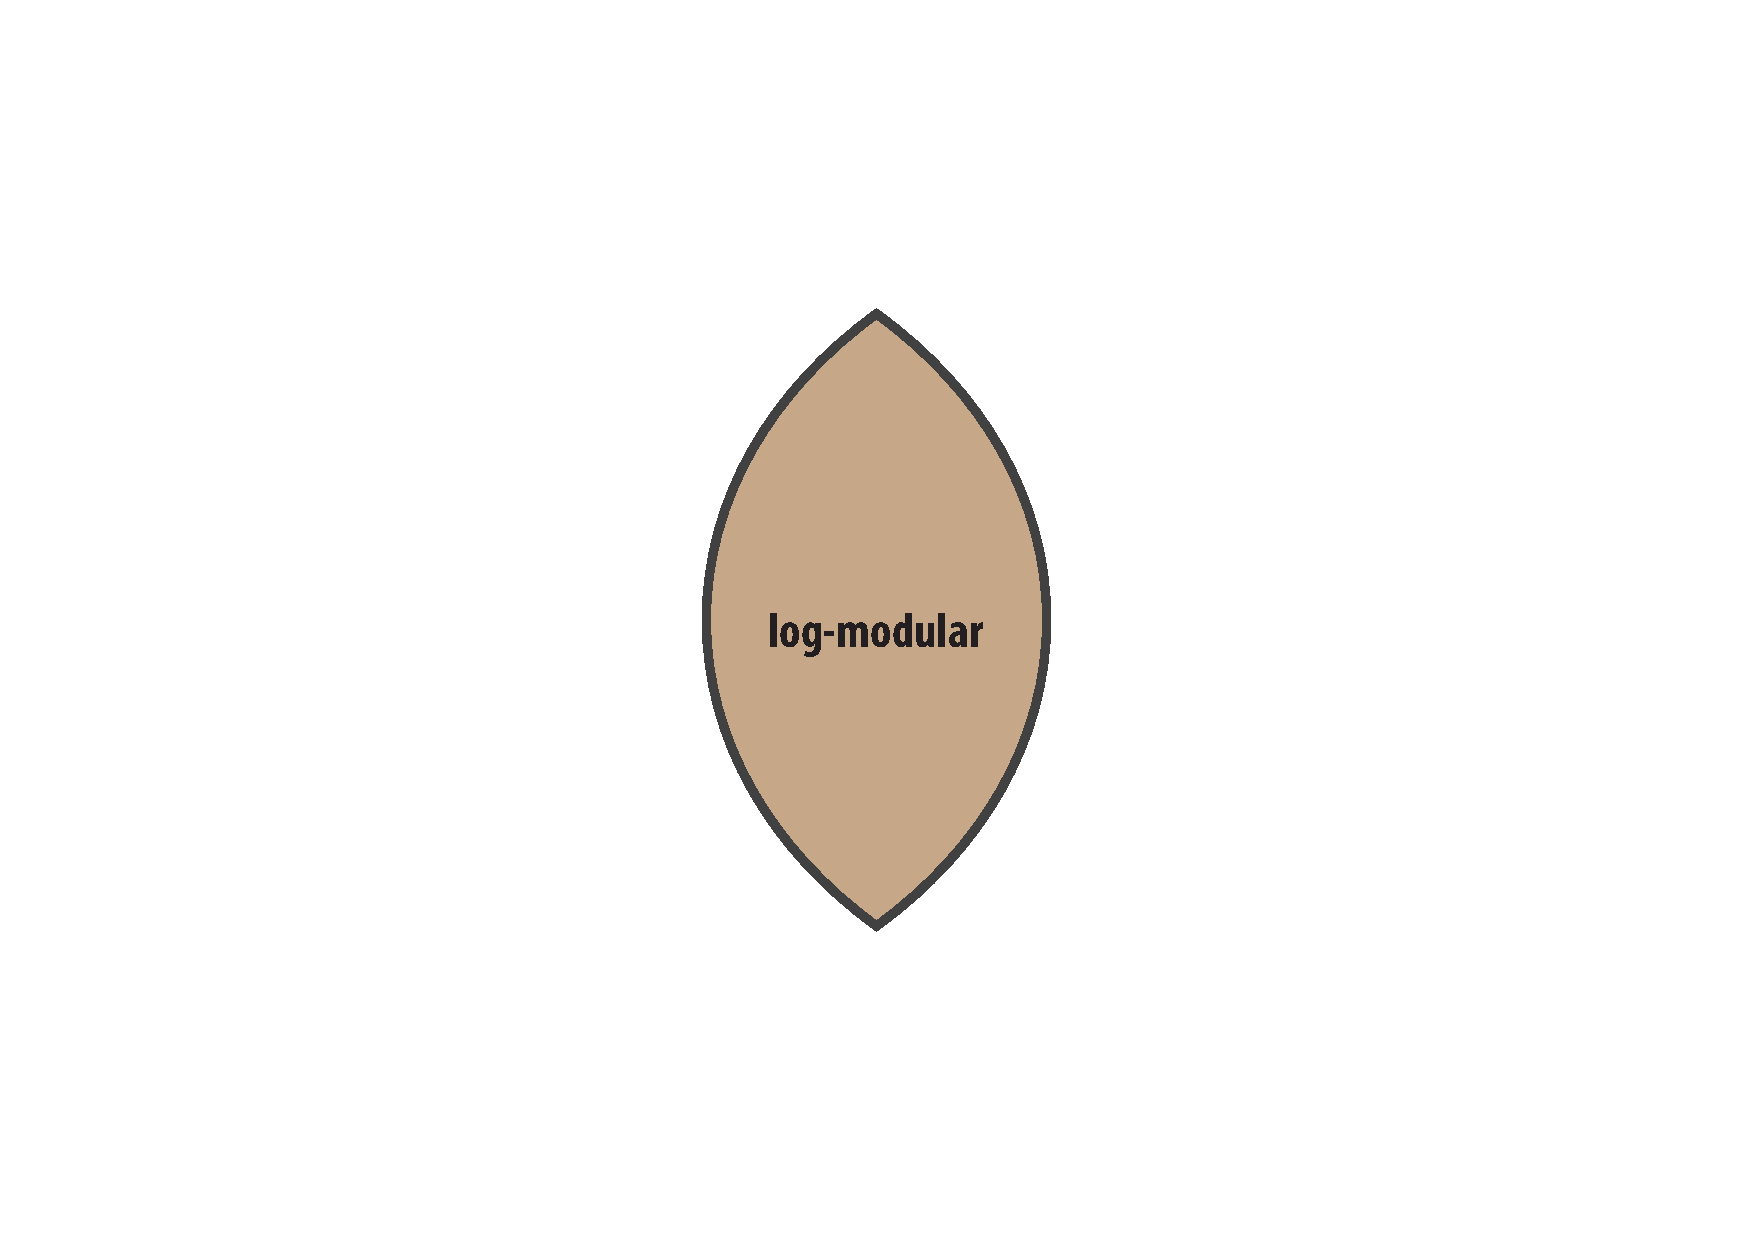
\includegraphics[width=4.3in]{figures/venn01.pdf}
\end{frame}

\begin{frame}{Landscape of Models}
\centering
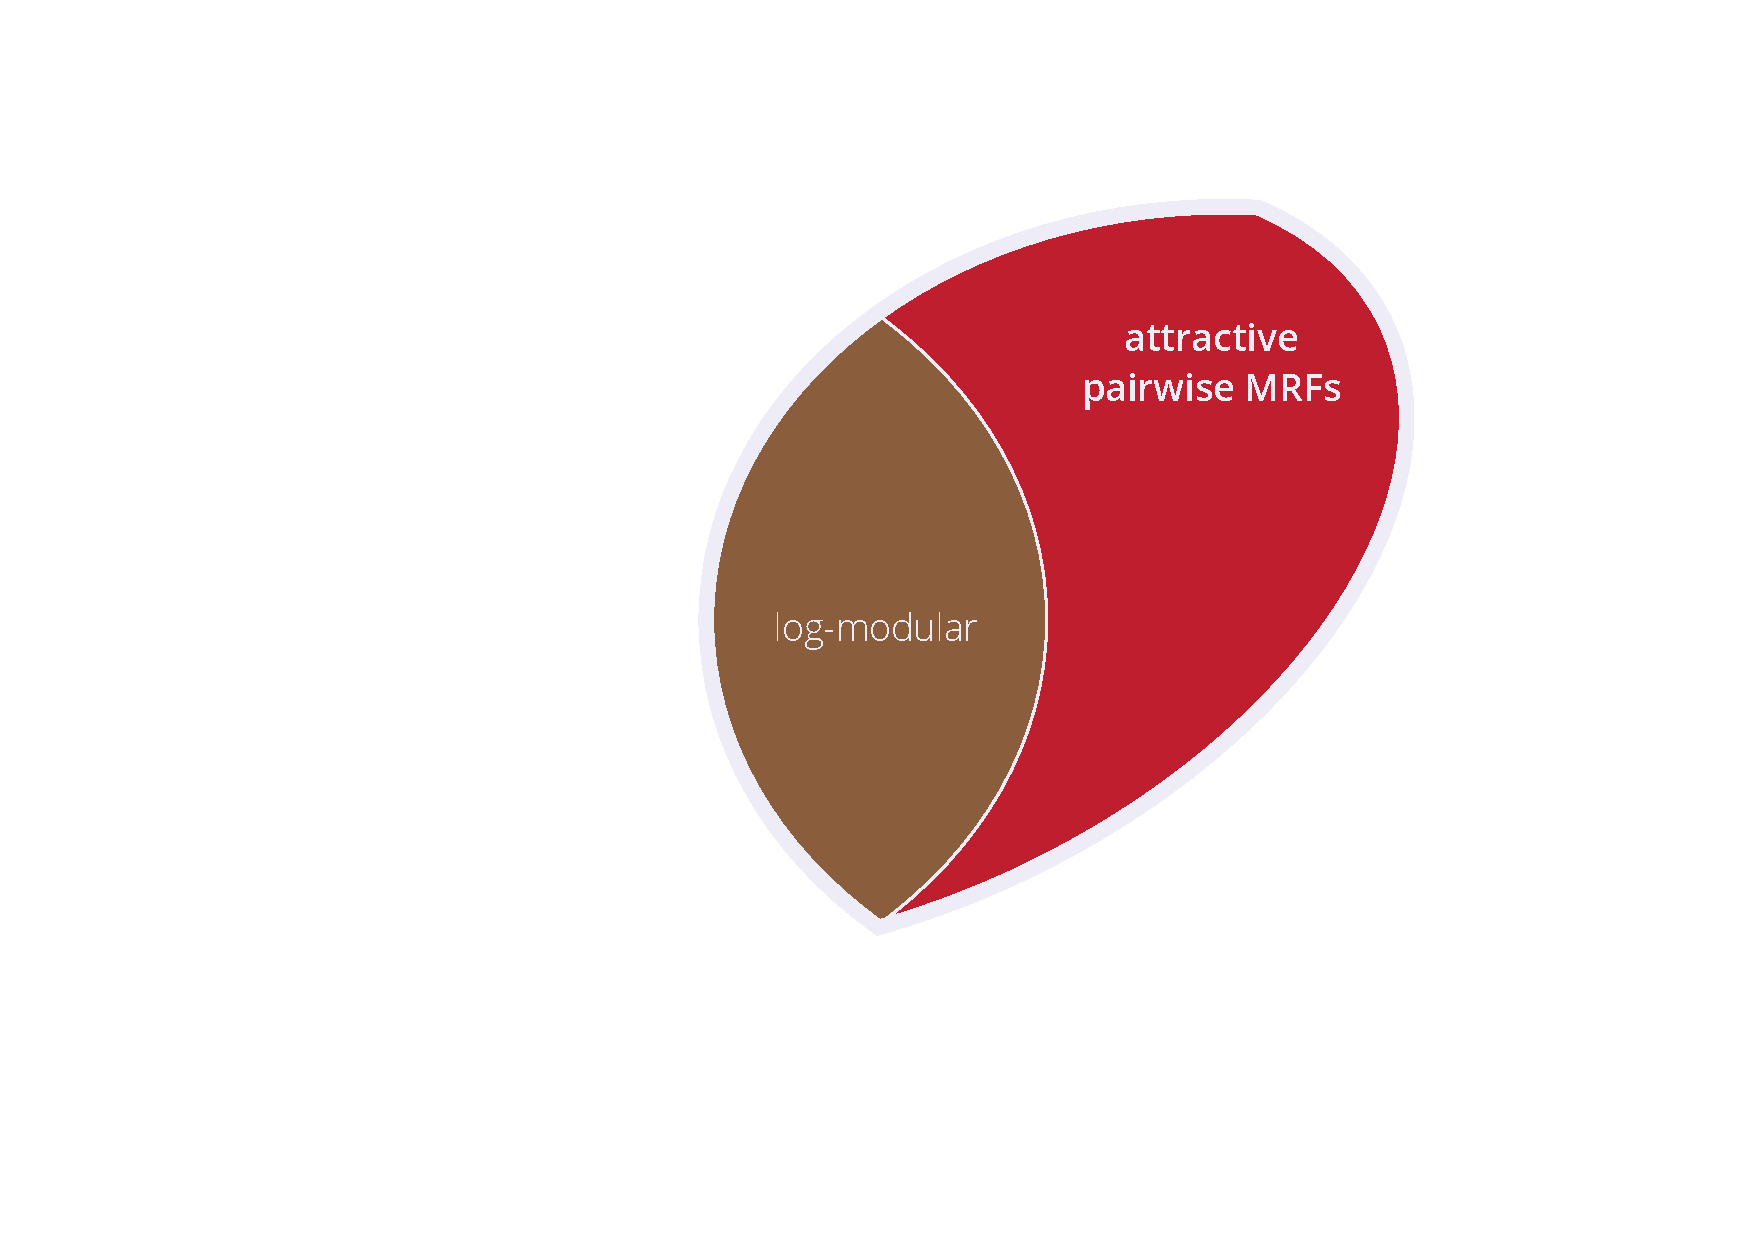
\includegraphics[width=4.3in]{figures/venn02.pdf}
\end{frame}

\begin{frame}{Landscape of Models}
\centering
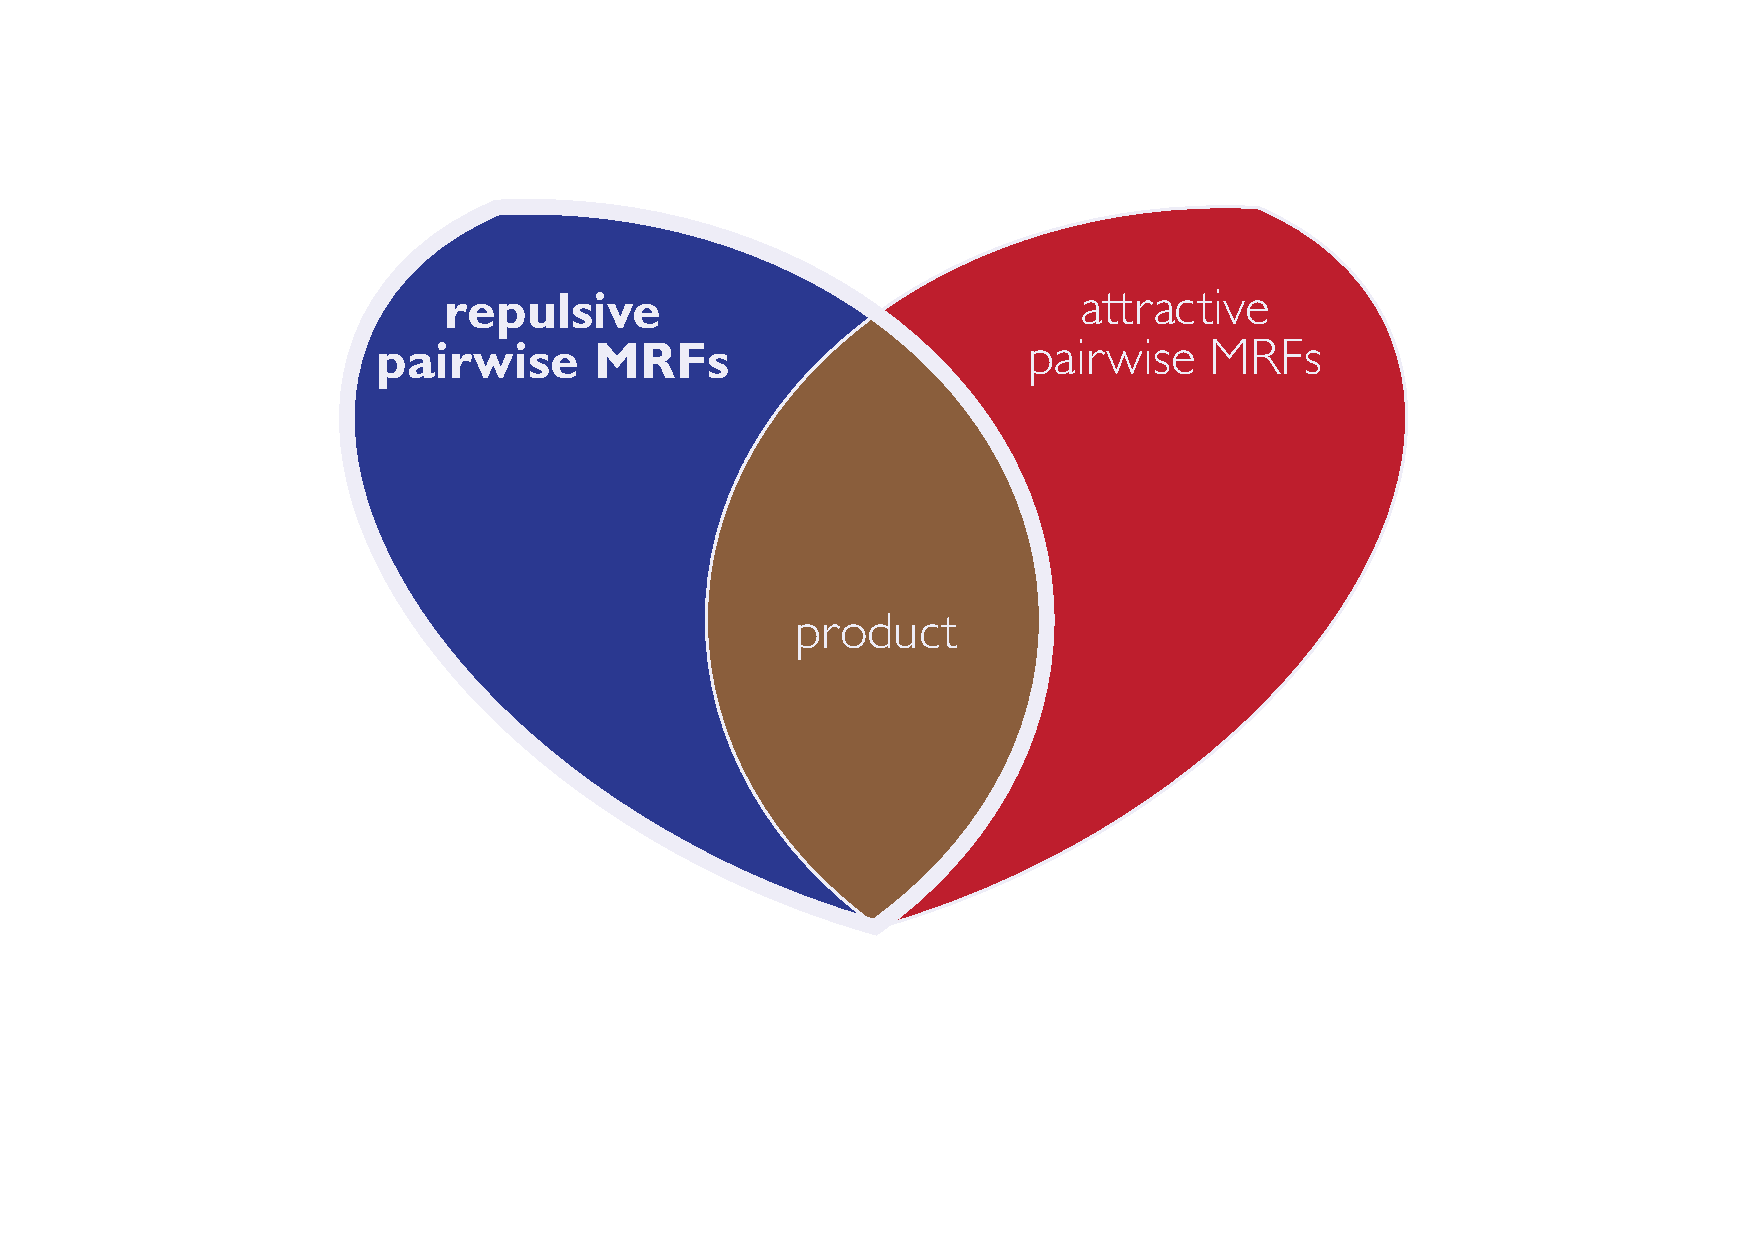
\includegraphics[width=4.3in]{figures/venn03.pdf}
\end{frame}

\begin{frame}{Landscape of Models}
\centering
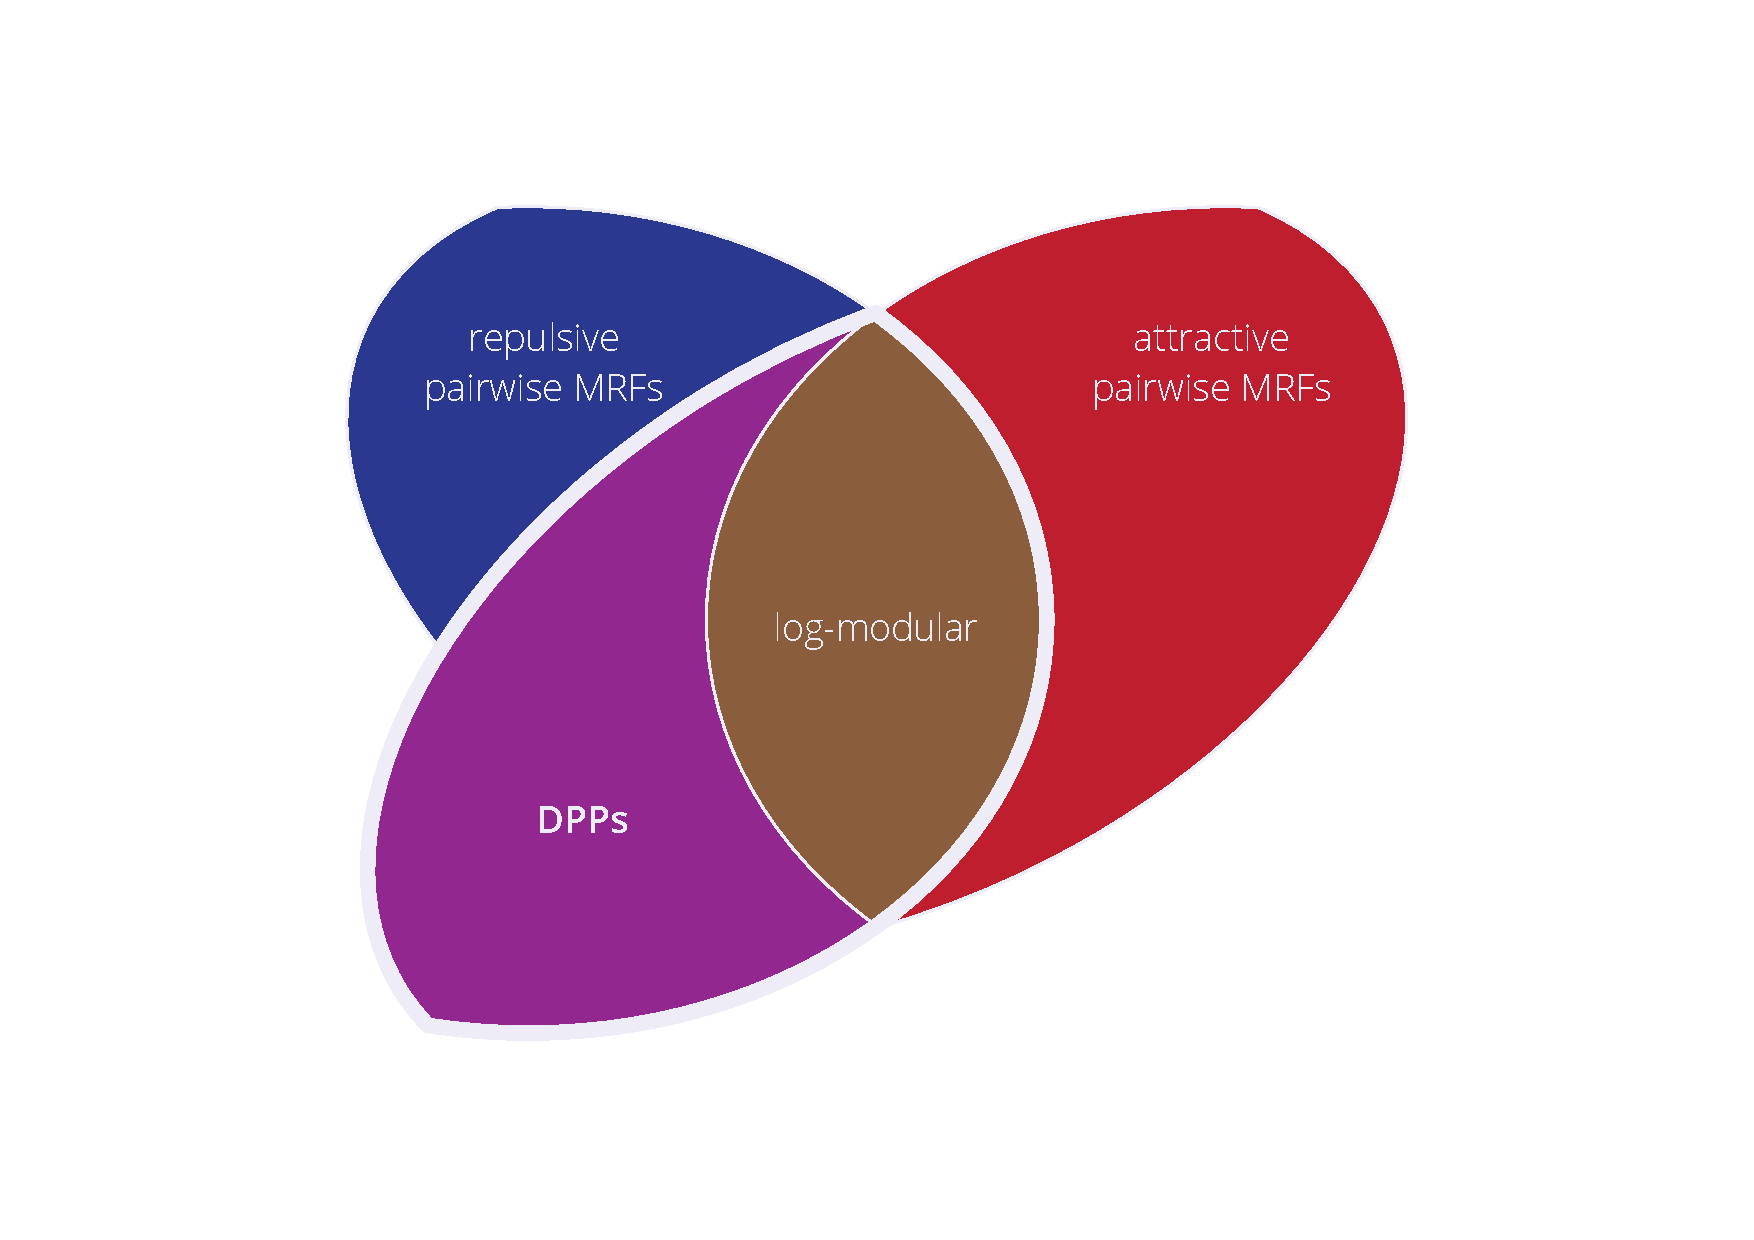
\includegraphics[width=4.3in]{figures/venn04.pdf}
\end{frame}

\begin{frame}{Landscape of Models}
\centering
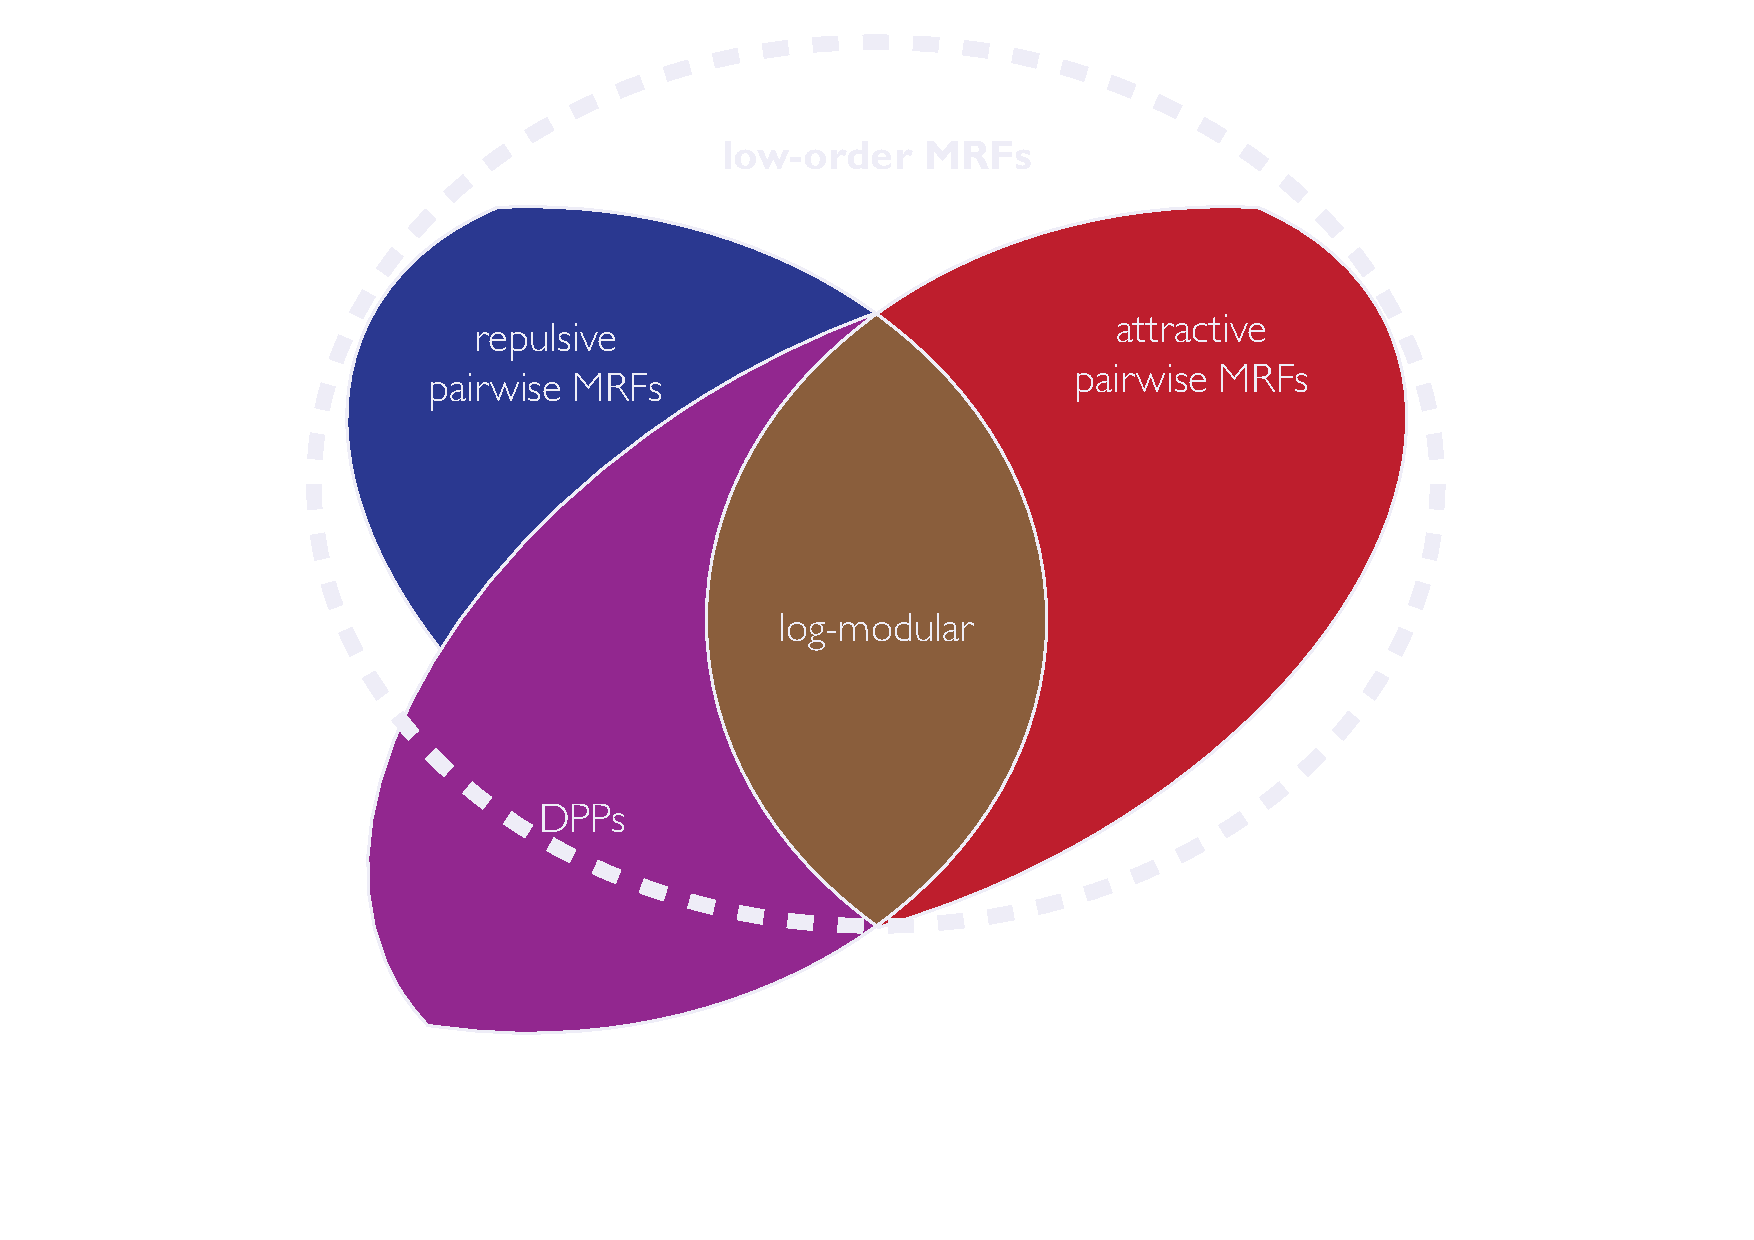
\includegraphics[width=4.3in]{figures/venn05.pdf}
\end{frame}

\begin{frame}{Landscape of Models}
\centering
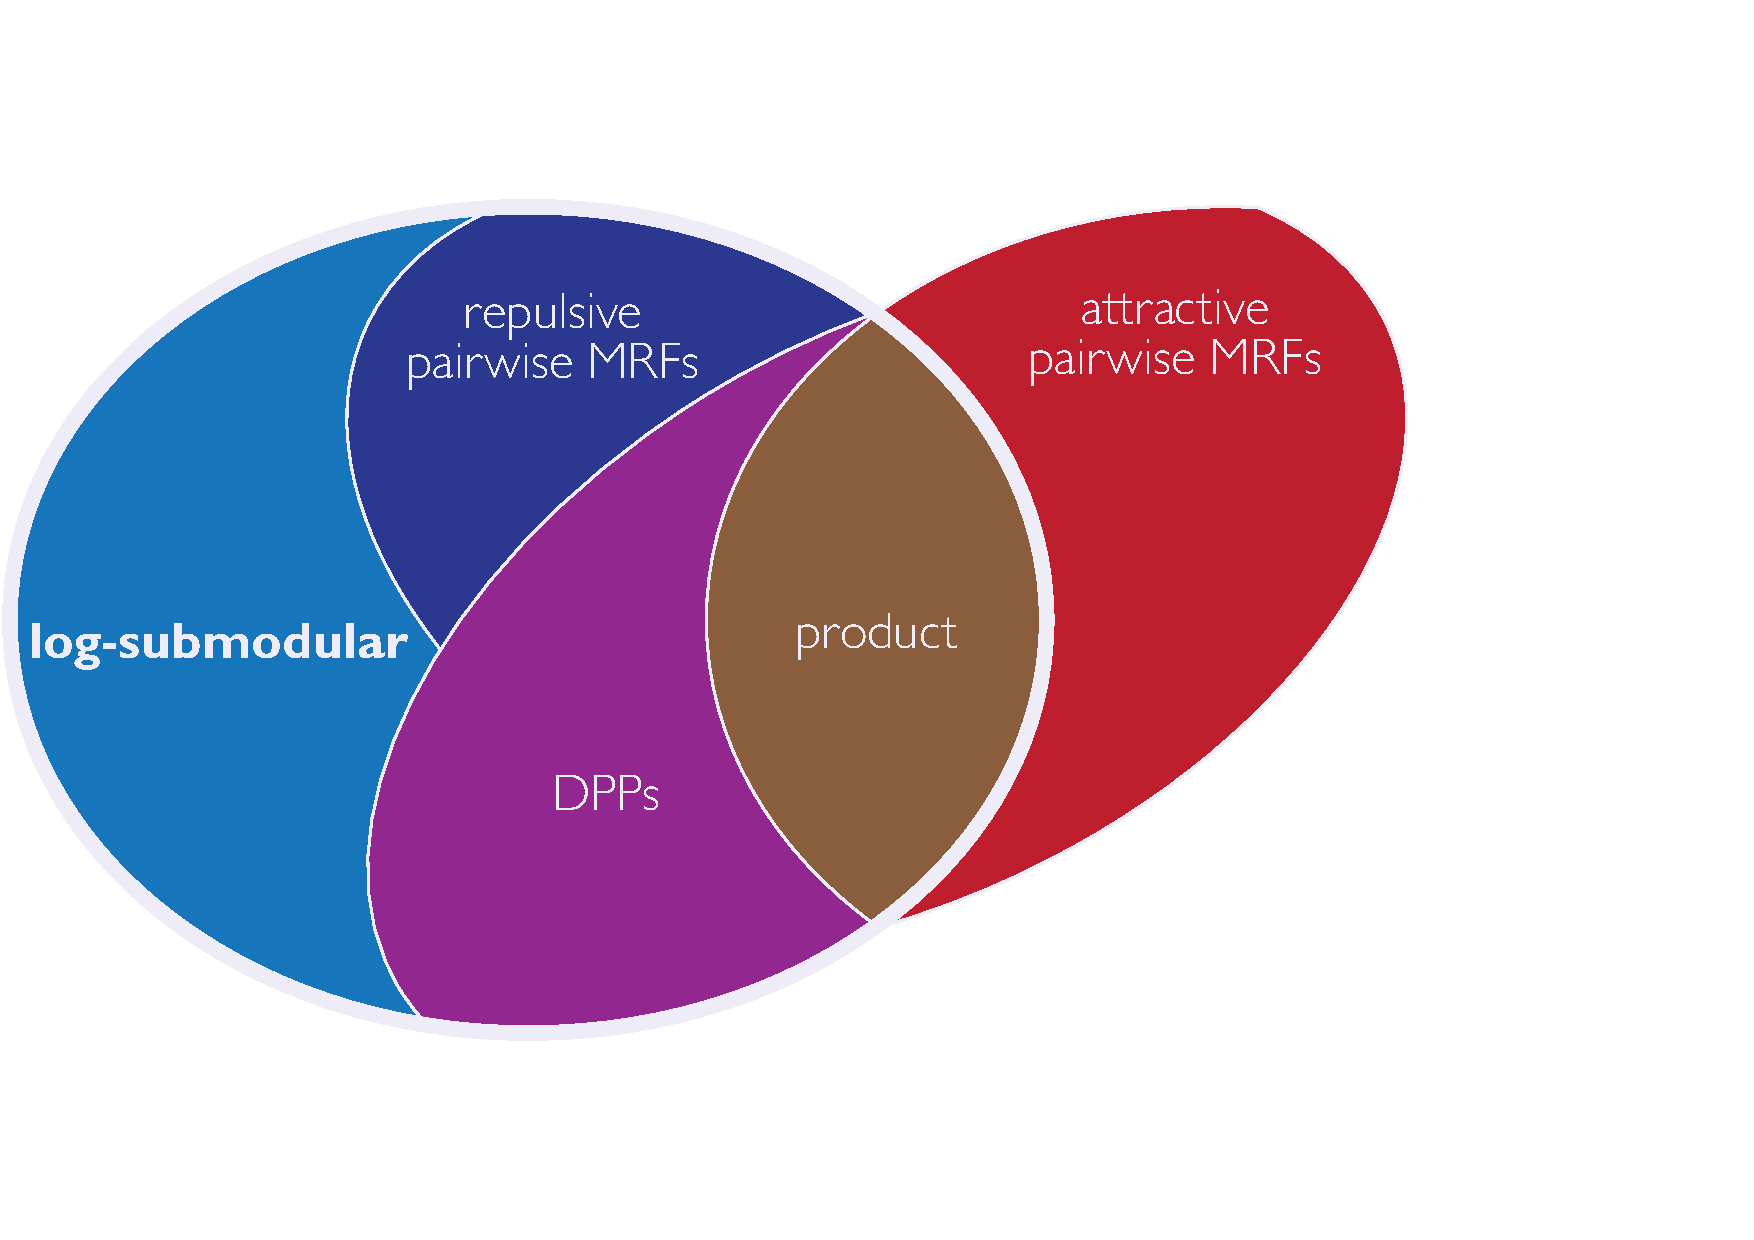
\includegraphics[width=4.3in]{figures/venn06.pdf}
\end{frame}

\begin{frame}{Landscape of Models}
\centering
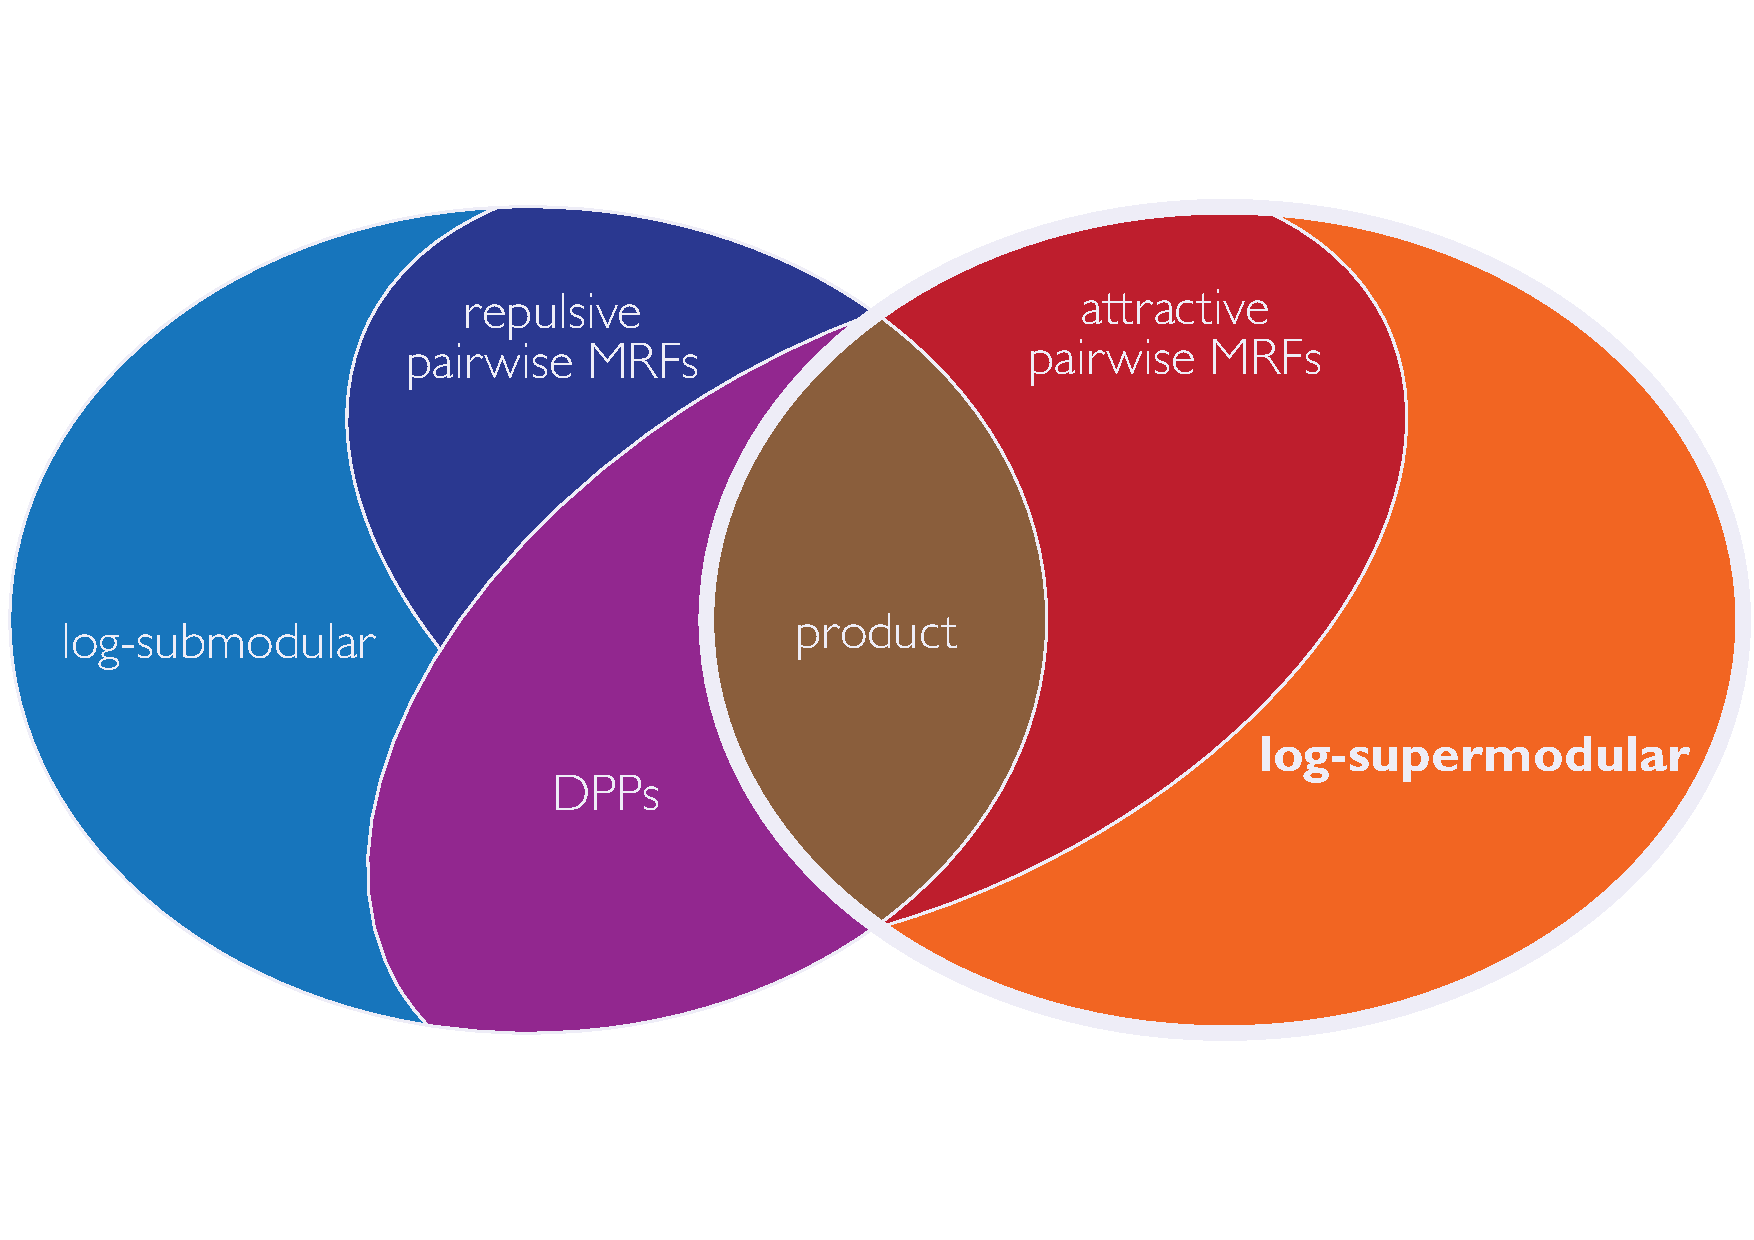
\includegraphics[width=4.3in]{figures/venn07.pdf}
\end{frame}

\begin{frame}{Landscape of Models}
\centering
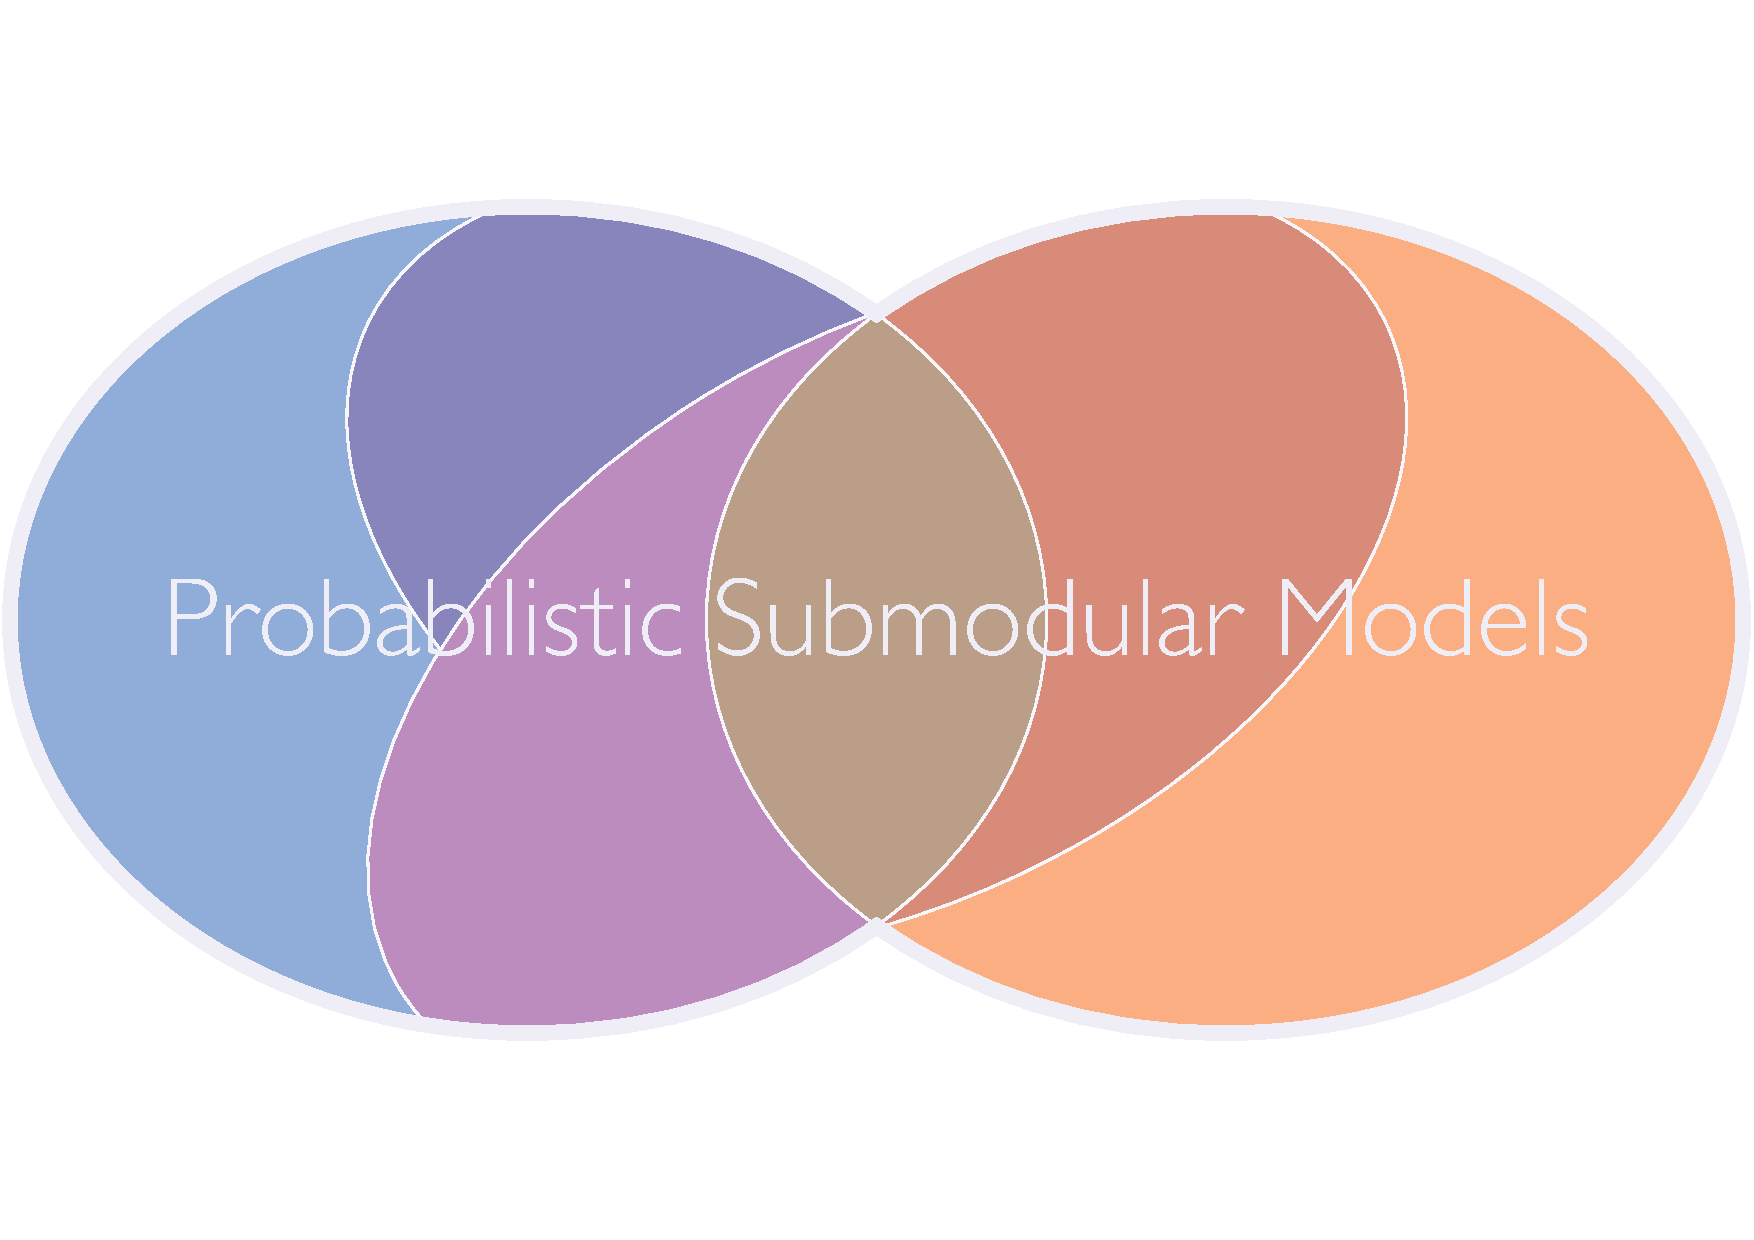
\includegraphics[width=4.3in]{figures/venn08.pdf}
\end{frame}

\end{document}
